\chapter{Logica di Floyd-Hoare}

Lo scopo della \fancyglitter{verifica dei programmi} è il controllo della soddisfacibilità delle specifiche, ossia che il programma sia \fancyglitter{corretto} e \fancyglitter{compilante}. Negli anni '60 Floyd propose di inserire delle formule logiche nei flow-chart dei programmi e Hoare introdusse le \fancyglitter{triple}\footnote{Accennate nel capitolo precedente.}.

\begin{center}
 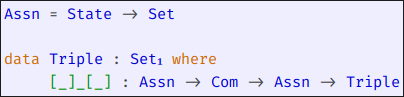
\includegraphics[scale = 0.5]{images/IMP/Assn.png}
\end{center}

\nt{Il tipo \texttt{Set}$_1$ è l'\fancyglitter{universo} più piccolo tale che \texttt{Set} = \texttt{Set}$_0$ : \texttt{Set}$_1$.}



\section{Il sistema della logica di Hoare}

\dfn{Logica di Hoare}{
  La logica di Hoare è un'assiomatizzazione della nozione di correttezza parziale. Consiste di un sistema formale di regole di inferenza i cui giudizi sono triple più formule logiche.
}

\cor{Asserzione}{Un'asserzione è un predicato dello stato.}

\cor{Tripla}{Una tripla \{P\} c \{Q\} significa che: quando in un certo stato vale la \textit{precondizione} P e l'esecuzione del \textit{comando} c in quello stato termina viene prodotto un nuovo stato che soddisfa la \textit{postcondizione} Q.

  In modo formale: se \textit{P s} e \textit{((c, s)) $\rightarrow$ t} allora \textit{Q t}.
}

\qs{}{Quando un'asserzione è valida?}

\paragraph{Risposta:} un'asserzione è valida quando è vera in tutti gli stati. 

\subsection{Regole}

\begin{center}
 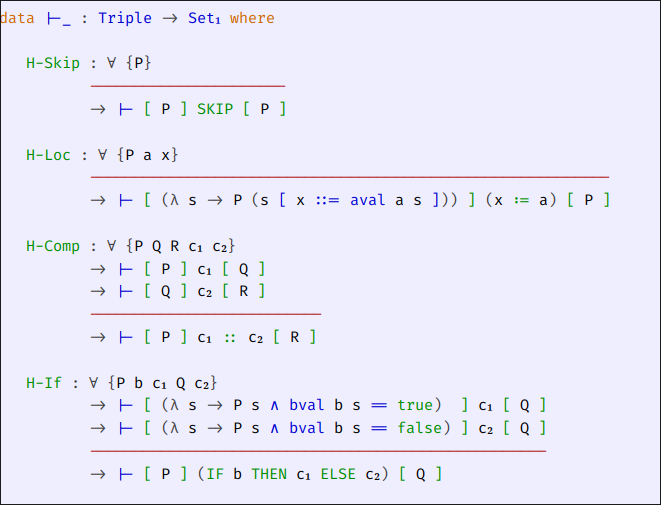
\includegraphics[scale = 0.4]{images/IMP/T1}
\end{center}

\begin{center}
 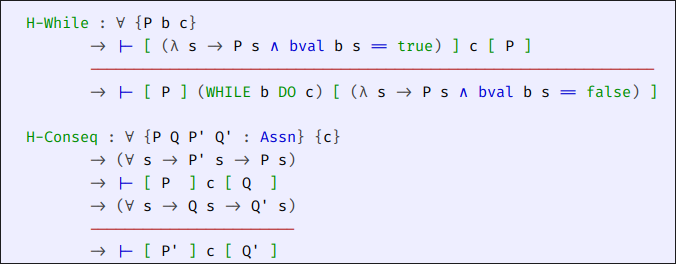
\includegraphics[scale = 0.4]{images/IMP/T2}
\end{center}

\dfn{Regole}{
  \begin{itemize}
    \item [$\Rightarrow$] H-Skip: è un'assioma. P è sia precondizione che postcondizione;
    \item [$\Rightarrow$] H-Loc: l'assegnazione, anche questo è un'assioma. Nella logica di Hoare si ragiona al rovescio, dalla postcondizione alla precondizione. Si vuole garantire la postcondizione P, per cui prima deve valere la precondizione P, ma nello stato precedente; 
    \item [$\Rightarrow$] H-Comp: si utilizza la transitività avendo un predicato intermedio tra i due comandi;
    \item [$\Rightarrow$] H-If: IF THEN ELSE esegue un comando diverso a seconda della precondizione, ossia se il booleano è vero o falso, ma alla fine la postcondizione è sempre Q;
    \item [$\Rightarrow$] H-While: al termine del while la guardia deve essere diventata falsa. Per cui nella precondizione vale sia P che la guardia b;
    \item [$\Rightarrow$] H-Conseq: P è un \textit{indebolimento} (implicato da un certo P') e Q è un \textit{rafforzamento} (implica un certo Q'). 
  \end{itemize}
}

\nt{Per via della nostra definizione di asserzione ci sono alcune differenze con le regole originali.}

\subsection{Regole derivate}

\begin{center}
 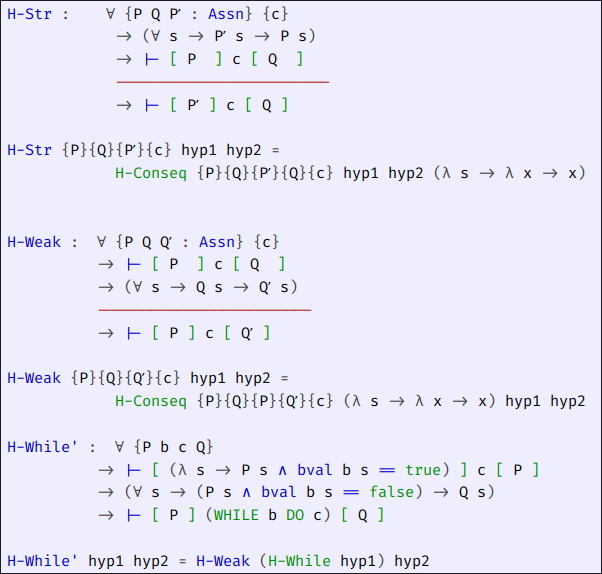
\includegraphics[scale = 0.4]{images/IMP/T3}
\end{center}

\dfn{Regole derivate}{
  \begin{itemize}
    \item [$\Rightarrow$] H-Str: specializzazione della conseguenza in cui la precondizione viene rafforzata;
    \item [$\Rightarrow$] H-Weak: specializzazione della conseguenza in cui la postcondizione viene indebolità;
    \item [$\Rightarrow$] H-While': è necessaria alla verifica semi-automatica dei programmi.    Si sfrutta la regola per il while in combinazione con l'indebolimento.
 
\end{itemize}
}

\section{Esempi}

\subsection{Assegnamento}

\begin{center}
 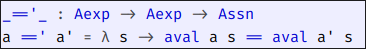
\includegraphics[scale = 0.6]{images/IMP/Ug}
 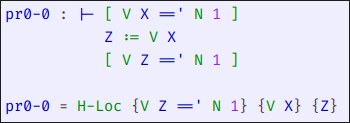
\includegraphics[scale = 0.6]{images/IMP/pr0-0}
 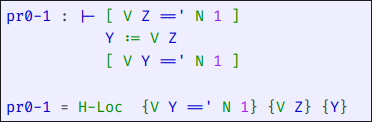
\includegraphics[scale = 0.6]{images/IMP/pr0-1}
\end{center}

\nt{La pre-condizione X = 1 è il risultato della sostituzione di Z con X nella post-condizione Z = 1. Dato che il comando termina sempre e assegna il valore di X a Z la tripla è valida (secondo il nostro formalismo \fancyglitter{H-Loc}).}

\subsection{Composizione}

\begin{center}
 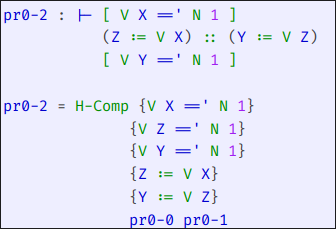
\includegraphics[scale = 0.6]{images/IMP/pr0-2}
\end{center}

\nt{Basta applicare la regola \fancyglitter{H-Comp} a pr0-0 e pr0-1.}

\subsection{Selezione}

Consideriamo \{T\} IF X $<$ Y THEN Z := Y ELSE Z := X \{Z = max(X,Y)\}\{T\} IF X $<$ Y THEN Z := Y ELSE Z := X \{Z = max(X,Y)\} (T è sempre vera, triviale). Per dimostrarla dobbiamo prima dimostrare:

\begin{center}
  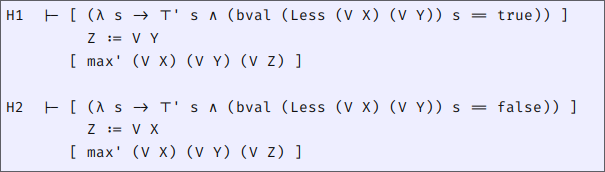
\includegraphics[scale = 0.5]{images/IMP/Ipotesi}
\end{center}

\begin{center}
  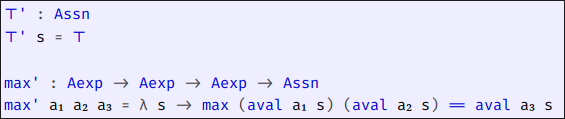
\includegraphics[scale = 0.5]{images/IMP/T-max}
\end{center}

\nt{max è $\bbN \to \bbN \to \bbN$ ed è definita nella libreria Nat.agda.}

\begin{center}
  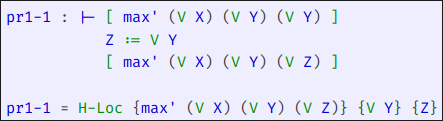
\includegraphics[scale = 0.4]{images/IMP/pr1-1}
  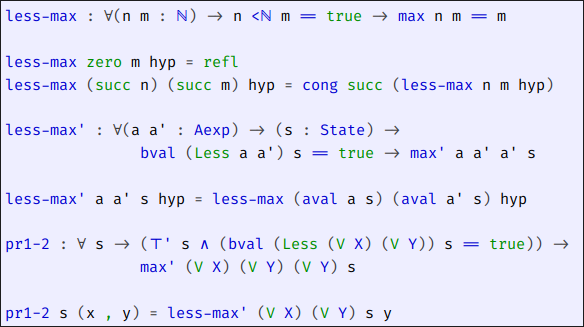
\includegraphics[scale = 0.4]{images/IMP/pr1-2}
\end{center}

\nt{Ora si può provare H1 mediante la regola di rafforzamento (\fancyglitter{H-STR}).}

\begin{center}
  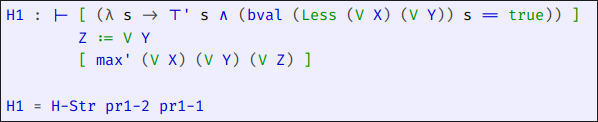
\includegraphics[scale = 0.5]{images/IMP/H1}
\end{center}

\nt{In maniera simile possiamo provare H2.}


\begin{center}
  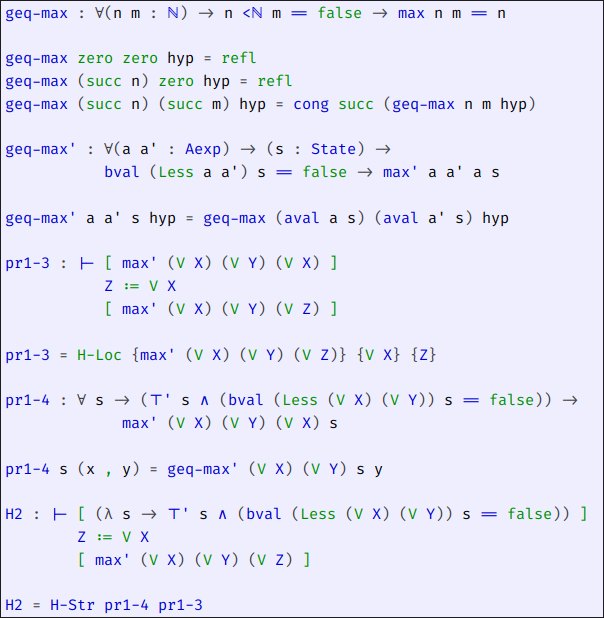
\includegraphics[scale = 0.5]{images/IMP/H2}
\end{center}

\nt{Infine si applica \fancyglitter{H-IF} alle ipotesi.}


\begin{center}
  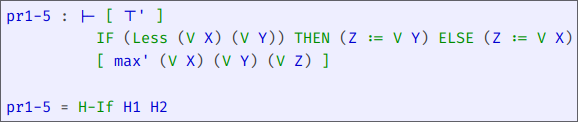
\includegraphics[scale = 0.5]{images/IMP/pr1-5}
\end{center}

\section{Correttezza}

\qs{}{Qual è la differenza tra \textit{vero} e \textit{valido}?}

\paragraph{Risposta:} in logica, vero si riferisce a un determinato modello con una determinata interpretazione, valido si riferisce a tutti i modelli. Nel contesto di questo corso il concetto di modello è sostituito dal concetto di stato, per cui una tripla è valida se è vera in tutti gli stati.

\begin{center}
  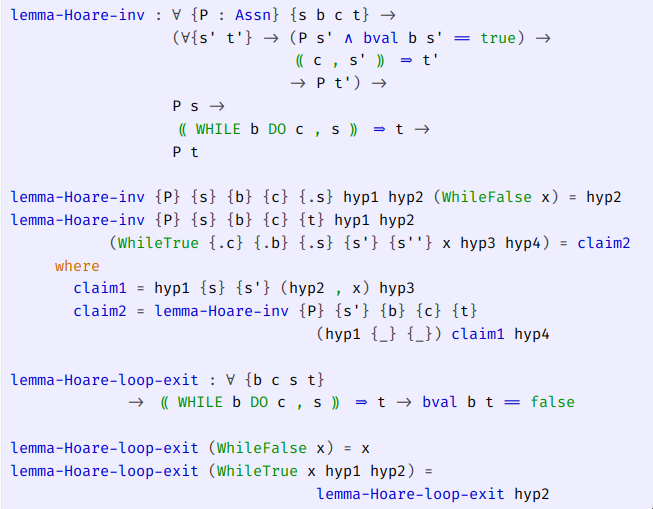
\includegraphics[scale = 0.5]{images/IMP/Inv.png}
\end{center}

\dfn{Cicli}{

  \begin{itemize}
    \item [$\Rightarrow$] lemma-Hoare-inv: stabilisce che quando P è vera e b anche (in s') se  c eseguito in s' produce t' e P è vera in t' allora la tripla [P] WHILE b DO c [P] è valida;
    \item [$\Rightarrow$] lemma-Hoare-loop-exit: gestisce l'uscita dal loop ossia la parte relativa alla valutazione di b come False al termine dell'esecuzione.
\end{itemize}

}

\begin{center}
  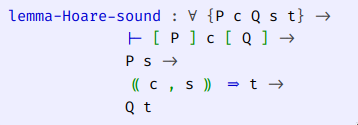
\includegraphics[scale = 0.6]{images/IMP/Sound.png}
\end{center}

\dfn{Lemma-Hoare-sound}{

  \begin{itemize}
    \item [$\Rightarrow$] caso SKIP: banalità, utilizza P s;
    \item [$\Rightarrow$] caso LOC: banalità, utilizza P s;
    \item [$\Rightarrow$] caso COMP: si applica l'ipotesi induttiva sia al primo elemento del COMP che al secondo (passandogli la prima ipotesi);
    \item [$\Rightarrow$] caso IF True: si applica l'ipotesi induttiva;
    \item [$\Rightarrow$] caso IF False: stesso procedimento usato per il true;
    \item [$\Rightarrow$] caso WHILE: si utilizza il lemma-Hoare-inv applicato all'ipotesi induttiva e il lemma-Hoare-exit applicato al comando;
    \item [$\Rightarrow$] caso CONSEQ: semplice applicazione dell'ipotesi induttiva.
\end{itemize}

}

\pagebreak

\begin{center}
  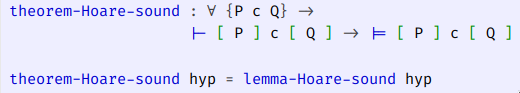
\includegraphics[scale = 0.5]{images/IMP/Sound2.png}
\end{center}

\dfn{Teorema-Hoare-sound}{Semplicemente si generalizza il lemma.}

\section{Completezza}

La completezza è l'implicazione inversa della completezza. 

\dfn{Completezza}{La completezza riguarda la capacità del sistema di catturare le cose vere. Se \{ P \} c \{ Q \} è valida allora è derivabile.}

\nt{Se il teorema di completezza fosse dimostrabile si avrebbe un'assiomatizzazione corretta dell'aritmetica, ma ciò andrebbe in contrasto con il primo teorema d'incompletezza di G\"odel. Tuttavia, in IMP è dimostrabile perché non è un sistema formale (per via della regola H-Conseq).}

\subsection{Weakest Liberal Precondition}

\begin{center}
  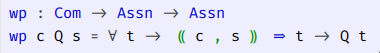
\includegraphics[scale = 0.5]{images/IMP/wlp.png}
\end{center}

\dfn{Weakest Liberal Precondition}{
  Le Weakest Liberal Preconditio prendono un comando, un'asserzione e restituiscono un'asserzione. L'idea è: dato un comando e data una postcondizione si vuole risalire alla precondizione più debole. Questo perché altrimenti non si potrebbe fare direttamente induzione.
}

\cor{Condizione debole}{Una condizione è più debole rispetto agli altri se è valida in un numero maggiore di stati.}

\nt{La condizione più debole  è quella che vale in qualsiasi stato (e. g. 0 == 0). }

\begin{center}
  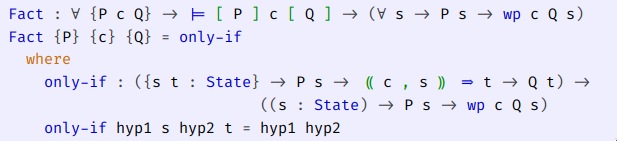
\includegraphics[scale = 0.5]{images/IMP/Fatto.png}
\end{center}

\dfn{Fatto}{
  Se \{ P \} c \{ Q \} è valido e ogni stato s soddisfa P allora è vero il wlp c Q s. 
}


\begin{center}
  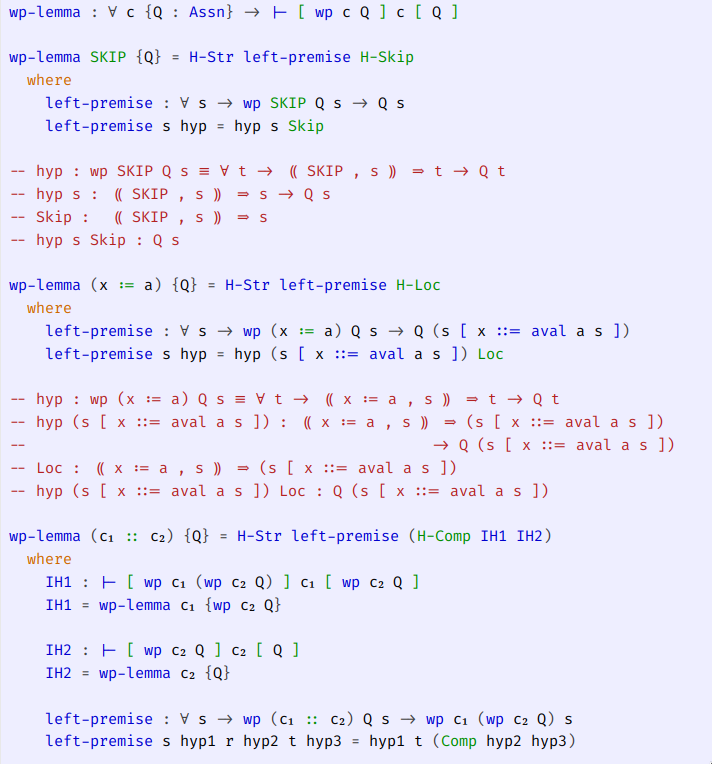
\includegraphics[scale = 0.5]{images/IMP/wlp1.png}
\end{center}

\dfn{Wlp-lemma - parte I}{
  \begin{itemize}
    \item [$\Rightarrow$] caso SKIP: la premessa da cui si parte consiste nella dimostrazione che wlp SKIP Q s implichi Q t. Per completare la dimostrazione si usa il rafforzamento con la premessa e la regola di Hoare per SKIP (H-Skip);
    \item [$\Rightarrow$] caso LOC: il procedimento è analogo a quello per SKIP;
    \item [$\Rightarrow$] caso COMP: si utilizza una composizione di funzioni. 
  \end{itemize}
}

\begin{center}
  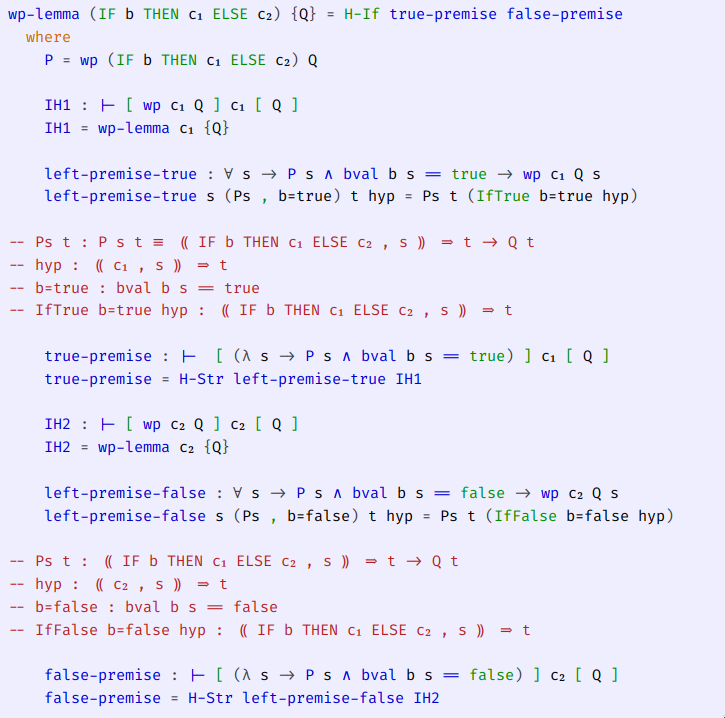
\includegraphics[scale = 0.5]{images/IMP/wlp2.png}
\end{center}

\dfn{Wlp-lemma - parte II}{
  \begin{itemize}
    \item [$\Rightarrow$] caso IF: si utilizzano due premesse, una per il caso in cui l'if sia vero e una per il caso in cui l'if sia falso.
  \end{itemize}
}

\begin{center}
  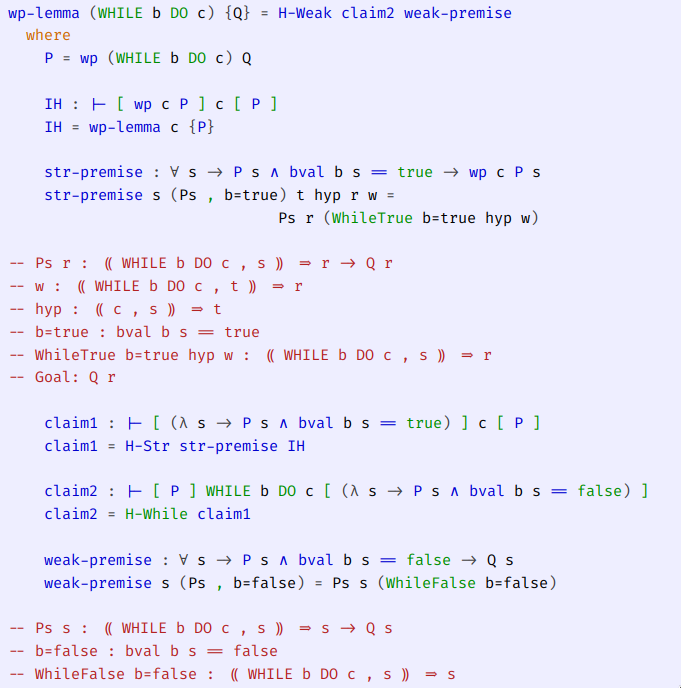
\includegraphics[scale = 0.5]{images/IMP/wlp3.png}
\end{center}

\dfn{Wlp-lemma - parte III}{
  \begin{itemize}
    \item caso WHILE: si sfrutta l'indebolimento per applicare la regola H-While applicaa a un rafforzamento dell'ipotesi induttiva.
  \end{itemize}
}

\begin{center}
  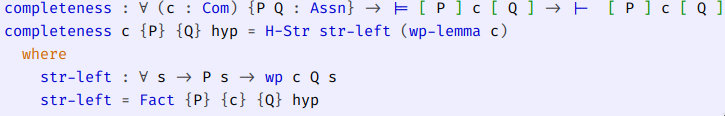
\includegraphics[scale = 0.5]{images/IMP/completezza.png}
\end{center}

\section{Verification Conditions}

\dfn{Verification Conditions}{}














